% Options for packages loaded elsewhere
\PassOptionsToPackage{unicode}{hyperref}
\PassOptionsToPackage{hyphens}{url}
%
\documentclass[
  ignorenonframetext,
  aspectratio=16,
]{beamer}
\usepackage{pgfpages}
\setbeamertemplate{caption}[numbered]
\setbeamertemplate{caption label separator}{: }
\setbeamercolor{caption name}{fg=normal text.fg}
\beamertemplatenavigationsymbolsempty
% Prevent slide breaks in the middle of a paragraph
\widowpenalties 1 10000
\raggedbottom
\setbeamertemplate{part page}{
  \centering
  \begin{beamercolorbox}[sep=16pt,center]{part title}
    \usebeamerfont{part title}\insertpart\par
  \end{beamercolorbox}
}
\setbeamertemplate{section page}{
  \centering
  \begin{beamercolorbox}[sep=12pt,center]{part title}
    \usebeamerfont{section title}\insertsection\par
  \end{beamercolorbox}
}
\setbeamertemplate{subsection page}{
  \centering
  \begin{beamercolorbox}[sep=8pt,center]{part title}
    \usebeamerfont{subsection title}\insertsubsection\par
  \end{beamercolorbox}
}
\AtBeginPart{
  \frame{\partpage}
}
\AtBeginSection{
  \ifbibliography
  \else
    \frame{\sectionpage}
  \fi
}
\AtBeginSubsection{
  \frame{\subsectionpage}
}
\usepackage{lmodern}
\usepackage{amssymb,amsmath}
\usepackage{ifxetex,ifluatex}
\ifnum 0\ifxetex 1\fi\ifluatex 1\fi=0 % if pdftex
  \usepackage[T1]{fontenc}
  \usepackage[utf8]{inputenc}
  \usepackage{textcomp} % provide euro and other symbols
\else % if luatex or xetex
  \usepackage{unicode-math}
  \defaultfontfeatures{Scale=MatchLowercase}
  \defaultfontfeatures[\rmfamily]{Ligatures=TeX,Scale=1}
\fi
% Use upquote if available, for straight quotes in verbatim environments
\IfFileExists{upquote.sty}{\usepackage{upquote}}{}
\IfFileExists{microtype.sty}{% use microtype if available
  \usepackage[]{microtype}
  \UseMicrotypeSet[protrusion]{basicmath} % disable protrusion for tt fonts
}{}
\makeatletter
\@ifundefined{KOMAClassName}{% if non-KOMA class
  \IfFileExists{parskip.sty}{%
    \usepackage{parskip}
  }{% else
    \setlength{\parindent}{0pt}
    \setlength{\parskip}{6pt plus 2pt minus 1pt}}
}{% if KOMA class
  \KOMAoptions{parskip=half}}
\makeatother
\usepackage{xcolor}
\IfFileExists{xurl.sty}{\usepackage{xurl}}{} % add URL line breaks if available
\IfFileExists{bookmark.sty}{\usepackage{bookmark}}{\usepackage{hyperref}}
\hypersetup{
  pdftitle={The Death and Life of Great British Cities},
  pdfauthor={Heblich; Nagy; Trew; Zylberberg},
  hidelinks,
  pdfcreator={LaTeX via pandoc}}
\urlstyle{same} % disable monospaced font for URLs
\newif\ifbibliography
\usepackage{graphicx}
\makeatletter
\def\maxwidth{\ifdim\Gin@nat@width>\linewidth\linewidth\else\Gin@nat@width\fi}
\def\maxheight{\ifdim\Gin@nat@height>\textheight\textheight\else\Gin@nat@height\fi}
\makeatother
% Scale images if necessary, so that they will not overflow the page
% margins by default, and it is still possible to overwrite the defaults
% using explicit options in \includegraphics[width, height, ...]{}
\setkeys{Gin}{width=\maxwidth,height=\maxheight,keepaspectratio}
% Set default figure placement to htbp
\makeatletter
\def\fps@figure{htbp}
\makeatother
\setlength{\emergencystretch}{3em} % prevent overfull lines
\providecommand{\tightlist}{%
  \setlength{\itemsep}{0pt}\setlength{\parskip}{0pt}}
\setcounter{secnumdepth}{-\maxdimen} % remove section numbering
\usepackage{pgfpages}
\usepackage{microtype}
\usepackage{tikz}
  \usetikzlibrary{positioning}
  \usetikzlibrary{arrows}
  \usetikzlibrary{graphs}

\definecolor{CTred}{RGB}{229,32,32}
\definecolor{CTgrey}{RGB}{153,153,153}


% colors: white text on 90% black background
\setbeamercolor{normal text}{fg=black,bg=white}

% light blue as a highlight color
\setbeamercolor*{structure}{fg=CTred}
\setbeamercolor{section title}{fg=CTred}
\setbeamercolor{alerted text}{use=structure,fg=CTred}
\setbeamercolor*{palette primary}{use=structure,fg=structure.fg}
\setbeamercolor*{palette secondary}{use=structure,fg=structure.fg!95!black}
\setbeamercolor*{palette tertiary}{use=structure,fg=structure.fg!90!black}
\setbeamercolor*{palette quaternary}{use=structure,fg=structure.fg!95!black,bg=black!80}

\setbeamercolor*{framesubtitle}{fg=white}


% use system fonts: here, Gill Sans
\usefonttheme{professionalfonts}
\setbeamerfont{quote}{shape=\upshape}

% eliminate silly beamer navigation line at bottom of slides
\setbeamertemplate{navigation symbols}{}

% ensure text jusfication
\usepackage{ragged2e}
\justifying

% pandoc makes 2nd-lever headers into blocks, and this ensures justification
% in blocks too
\addtobeamertemplate{block begin}{}{\justifying}




\urlstyle{same}
\usepackage[overlay,absolute]{textpos}

\setbeamertemplate{items}[square]

\TPGrid[10 mm,8 mm]{9}{8}
% beamer's left and right margin is 10 mm. The top/bottom margin is ??
% or without a header ??
% the slide dimensions are 128 mm x 96 mm
% so the resulting \TPHorizModule = 12 mm and \TPVertModule = 10 mm

% uncomment if you want biblatex for citations on slides

% \usepackage{csquotes}
% \usepackage[notes,short,noibid,backend=biber]{biblatex-chicago}
% \bibliography{course.bib} 

\providecommand{\exhibit}[2]{\includegraphics[keepaspectratio, height=0.9\textheight, width=\textwidth]{assets/img/#1}\\ {\tiny #2}}

\title{The Death and Life of Great British Cities}
\author{Heblich \and Nagy \and Trew \and Zylberberg}
\date{Discussion by Miklós Koren}

\begin{document}
\frame{\titlepage}

\begin{frame}{Outline}
\protect\hypertarget{outline}{}
\begin{enumerate}
\tightlist
\item
  One-page summary
\item
  Broader comments
\item
  One point about empirics
\item
  One point about theory
\end{enumerate}
\end{frame}

\begin{frame}{One-page summary}
\protect\hypertarget{one-page-summary}{}
Use 200 years of data from England and Wales.

Large, contiguous plots of land around the city are associated with:

\begin{itemize}
\tightlist
\item
  stronger specialization
\item
  fast population growth earlier, decline later
\end{itemize}
\end{frame}

\begin{frame}{Broader comments}
\protect\hypertarget{broader-comments}{}
Economies of scale, scope and density are most interesting in economics.

Big shifts in sectoral specialization, population, productivity and
economic geography likely related.

Spatial macroeconomics is promising not only for historical development.
\end{frame}

\hypertarget{one-point-about-empirics}{%
\section{One point about empirics}\label{one-point-about-empirics}}

\begin{frame}{One point about empirics}
\protect\hypertarget{one-point-about-empirics-1}{}
Meanshift algorithm clusters points in multidimensional space.

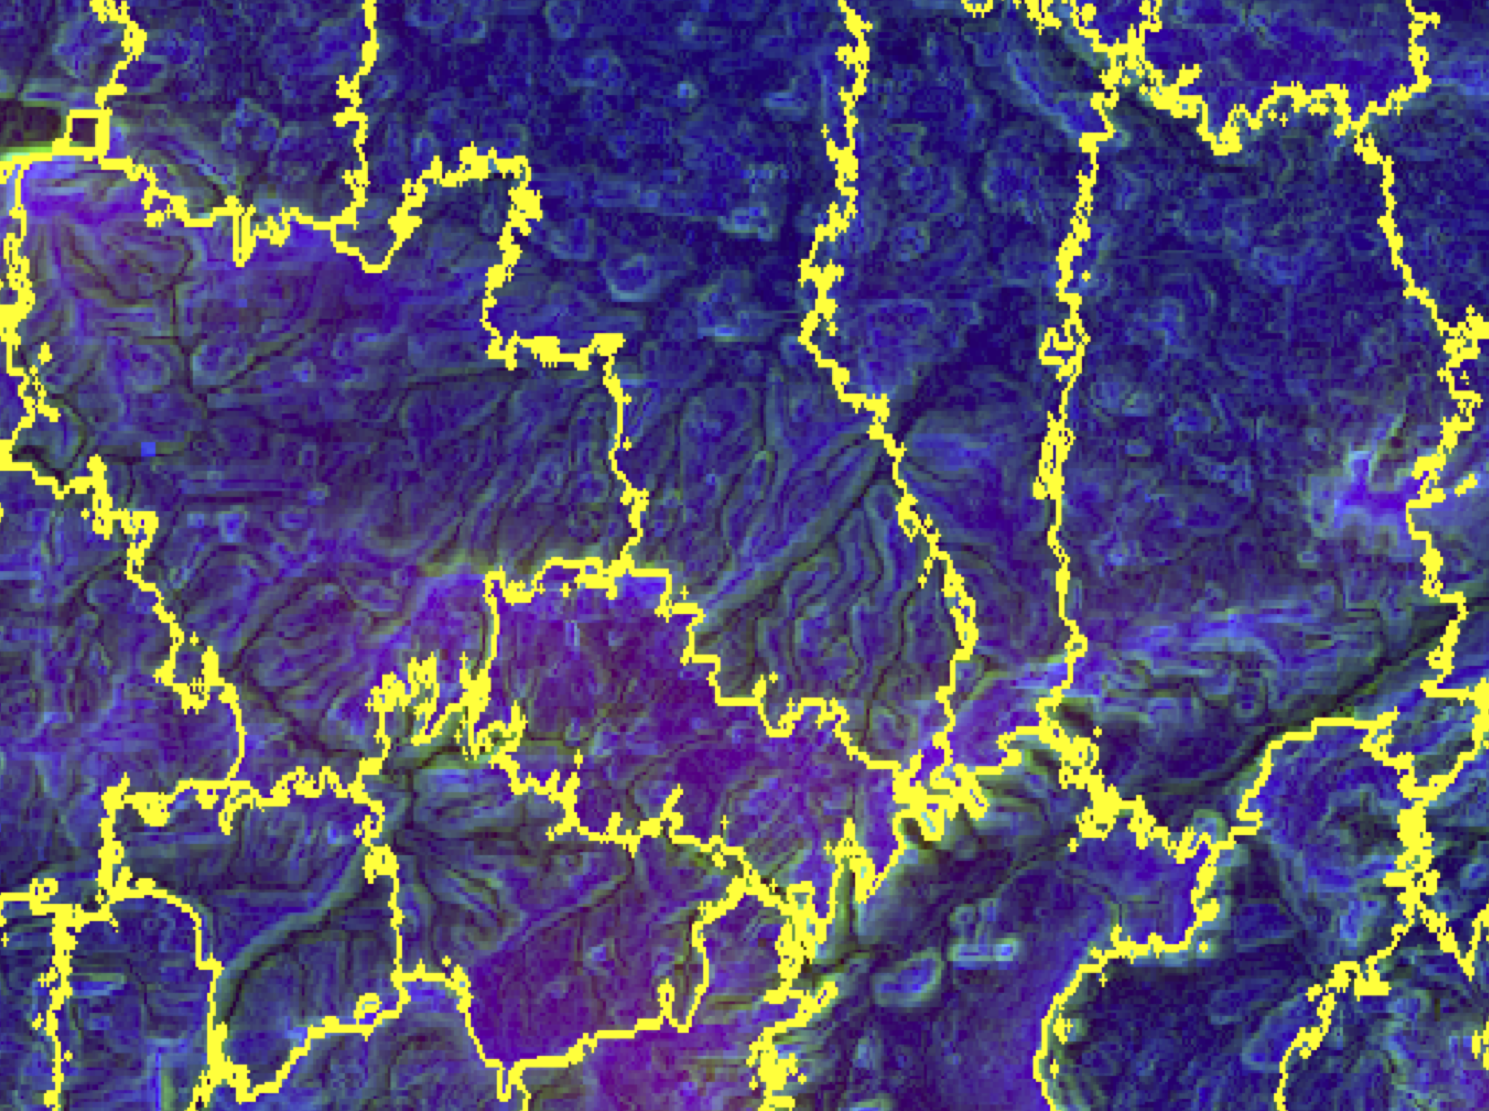
\includegraphics{clusters.png}

\begin{block}{But}
\protect\hypertarget{but}{}
Much depends on relative weights of other dimensions; need to know more.

Very few spatial data is truly raster; often based on vectoral data; can
be misleading.
\end{block}
\end{frame}

\begin{frame}{Example: WorldPop raster}
\protect\hypertarget{example-worldpop-raster}{}
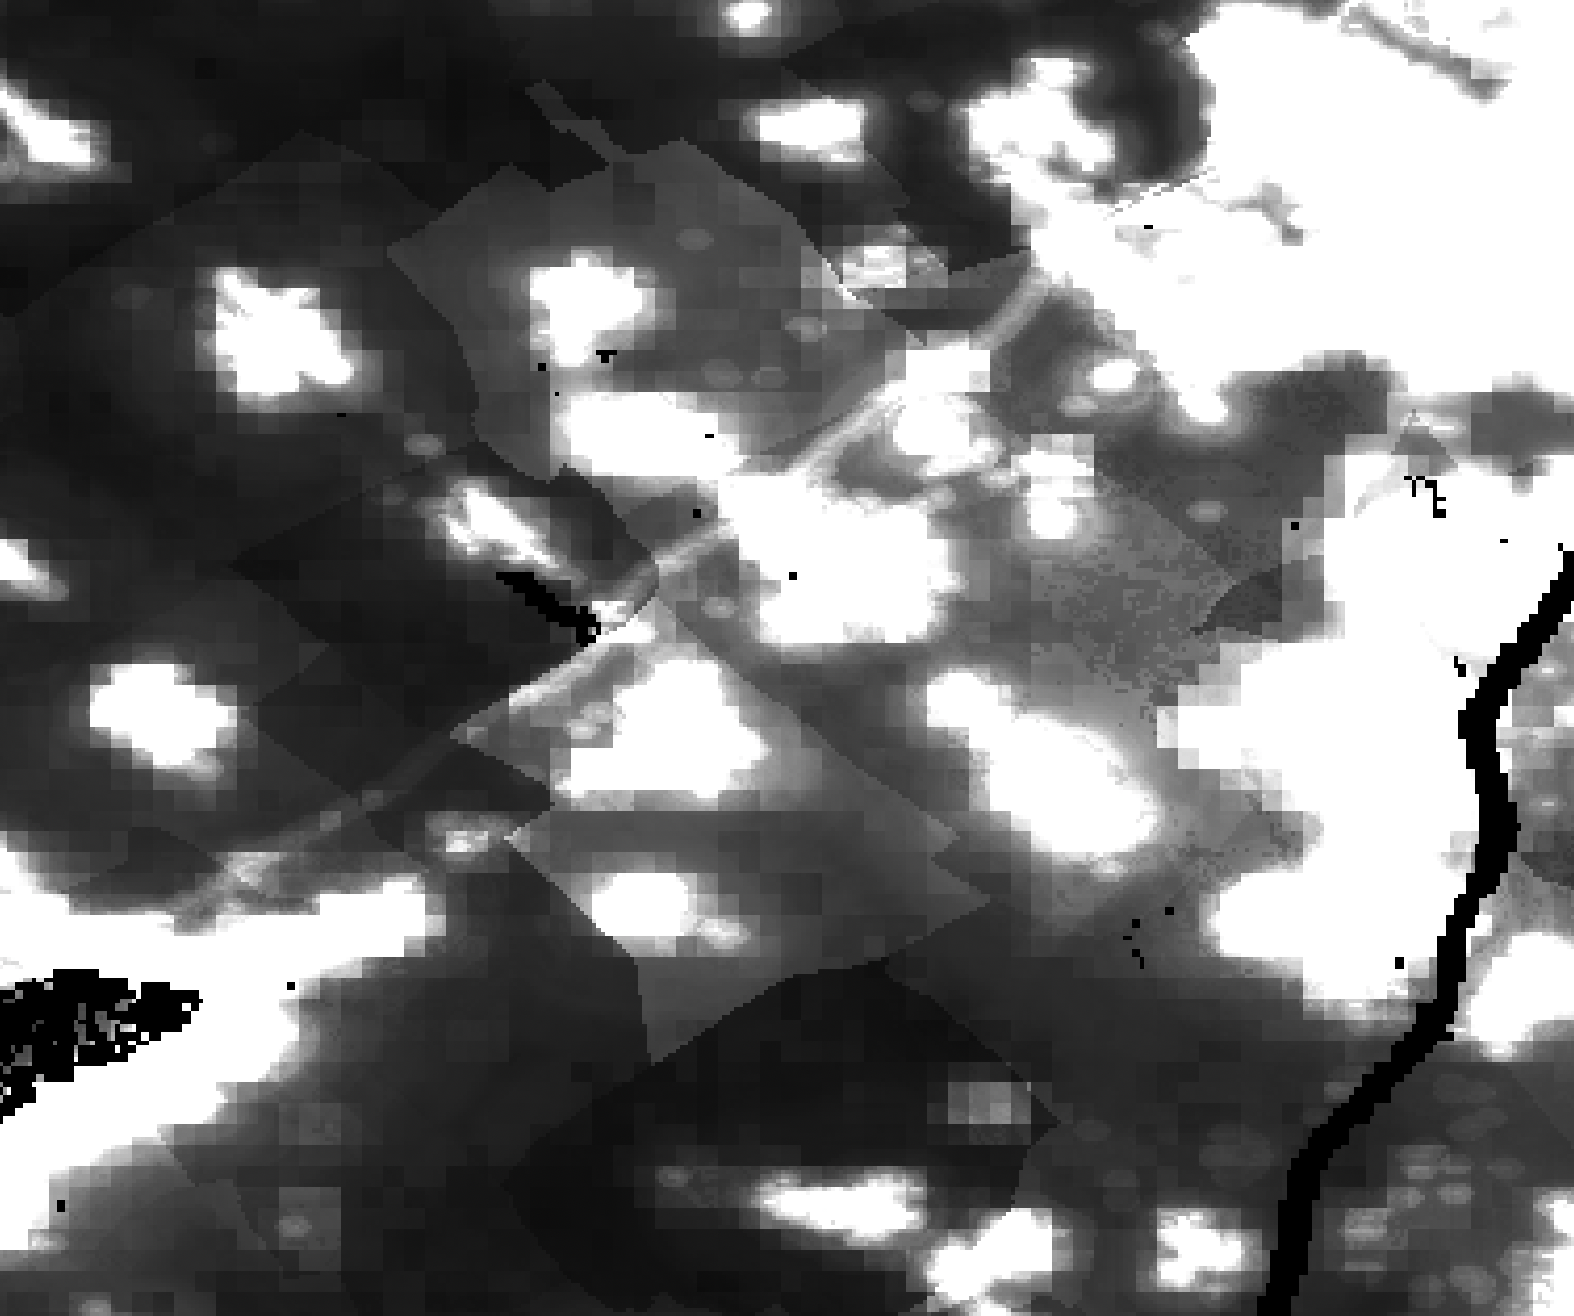
\includegraphics{raster.png}
\end{frame}

\begin{frame}{Example: OpenStreetMap vector}
\protect\hypertarget{example-openstreetmap-vector}{}
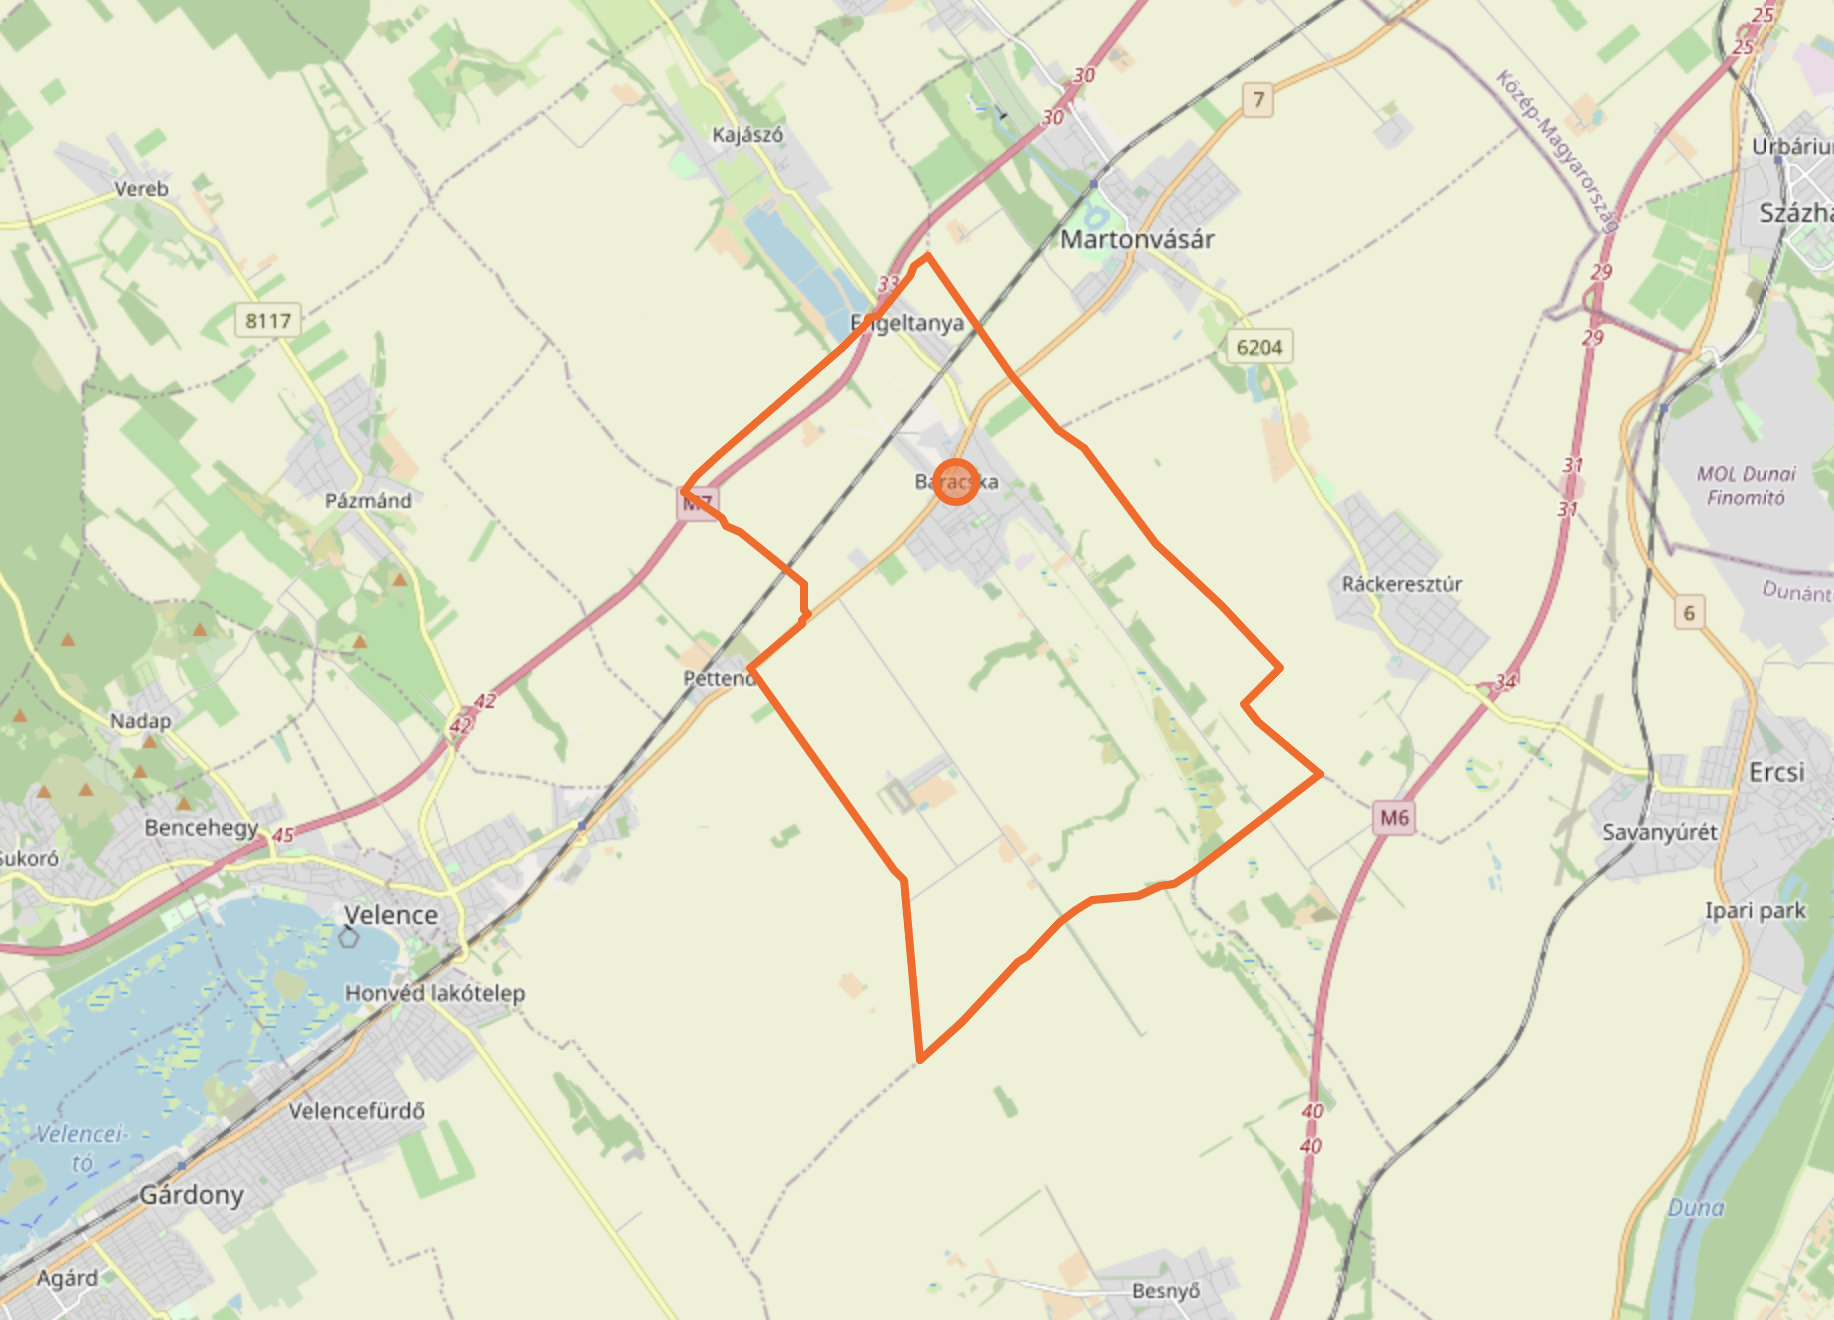
\includegraphics{vector.png}
\end{frame}

\begin{frame}{This is a problem for all top-down datasets}
\protect\hypertarget{this-is-a-problem-for-all-top-down-datasets}{}
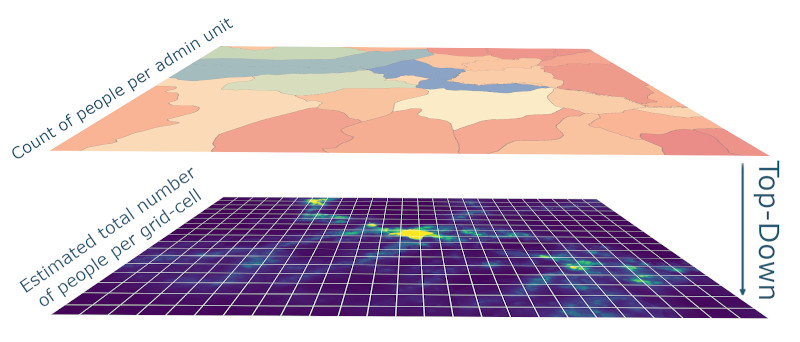
\includegraphics{topdown.jpg}
\end{frame}

\hypertarget{one-point-about-theory}{%
\section{One point about theory}\label{one-point-about-theory}}

\begin{frame}{One point about theory}
\protect\hypertarget{one-point-about-theory-1}{}
This is a reversal of fortune story. These stories are challenging for
neoclassical economics for two reasons:

\begin{enumerate}
\tightlist
\item
  contradict perfect foresight
\item
  contradict free disposal
\end{enumerate}
\end{frame}

\begin{frame}{Why are some cities bad that used to be good?}
\protect\hypertarget{why-are-some-cities-bad-that-used-to-be-good}{}
\begin{enumerate}
\tightlist
\item
  myopia or externalities
\item
  adjustment costs, irreversibilities, non-convexities

  \begin{itemize}
  \tightlist
  \item
    more relevant for heavy industry
  \item
    potentially relevant for spatial development
  \end{itemize}
\end{enumerate}
\end{frame}

\end{document}
